\documentclass[conference]{IEEEtran}
\IEEEoverridecommandlockouts
% The preceding line is only needed to identify funding in the first footnote. If that is unneeded, please comment it out.
\usepackage{cite}
\usepackage{amsmath,amssymb,amsfonts}
\usepackage{algorithmic}
\usepackage{graphicx}
\usepackage{textcomp}
\usepackage{xcolor}
\usepackage{url}
\usepackage{subcaption}
\usepackage{multirow}
\usepackage{booktabs}
\usepackage{listings}
\usepackage{xcolor}

% Define colors for syntax highlighting
\definecolor{codegreen}{rgb}{0,0.6,0}
\definecolor{codegray}{rgb}{0.5,0.5,0.5}
\definecolor{codepurple}{rgb}{0.58,0,0.82}
\definecolor{backcolour}{rgb}{0.95,0.95,0.92}

% Configure listings package
\lstdefinestyle{mystyle}{
    backgroundcolor=\color{backcolour},   
    commentstyle=\color{codegreen},
    keywordstyle=\color{magenta},
    numberstyle=\tiny\color{codegray},
    stringstyle=\color{codepurple},
    basicstyle=\ttfamily\footnotesize,
    breakatwhitespace=false,         
    breaklines=true,                 
    captionpos=b,                    
    keepspaces=true,                 
    numbers=left,                    
    numbersep=5pt,                  
    showspaces=false,                
    showstringspaces=false,
    showtabs=false,                  
    tabsize=2
}

\lstset{style=mystyle}

\def\BibTeX{{\rm B\kern-.05em{\sc i\kern-.025em b}\kern-.08em
    T\kern-.1667em\lower.7ex\hbox{E}\kern-.125emX}}

\begin{document}

\title{Comparative Analysis of Classical and Graph Neural Network Approaches for Community Detection in Citation Networks}

\author{\IEEEauthorblockN{Emre Yıldız}
\IEEEauthorblockA{\textit{Department of Computer Engineering} \\
\textit{Ege University}\\
İzmir, Turkey \\
emre.yildiz.dev@hotmail.com}
}

\maketitle

\begin{abstract}
Community detection in complex networks is a fundamental problem in network analysis with applications ranging from social network analysis to biological systems. This paper presents a comprehensive comparative study of classical community detection algorithms and modern Graph Neural Network (GNN) approaches applied to the Cora citation network dataset. We implement and evaluate three classical algorithms (Louvain and Label Propagation) alongside three GNN architectures (Graph Convolutional Networks, GraphSAGE, and Graph Attention Networks) in both supervised and unsupervised settings. Our experimental framework integrates Neo4j graph database for efficient data management and classical algorithm execution, while PyTorch Geometric provides the foundation for GNN implementations. Results demonstrate that semi-supervised GNN approaches significantly outperform classical methods, achieving Adjusted Rand Index scores of 0.87, 0.86, and 0.86 for GAT, GraphSAGE, and GCN respectively, compared to 0.24 and 0.15 for Louvain and Label Propagation algorithms. The study provides insights into the effectiveness of different approaches for community detection in academic citation networks.
\end{abstract}

\begin{IEEEkeywords}
community detection, graph neural networks, citation networks, Neo4j, Louvain algorithm, label propagation
\end{IEEEkeywords}

\section{Introduction}

Community detection is a crucial task in network analysis that aims to identify groups of nodes that are more densely connected to each other than to nodes in other groups. In the context of citation networks, communities often represent research areas or academic disciplines where papers within the same community share similar topics or methodologies.

The Cora dataset, consisting of 2,708 machine learning papers classified into seven categories (Neural Networks, Probabilistic Methods, Genetic Algorithms, Theory, Case-Based, Reinforcement Learning, and Rule Learning), provides an excellent benchmark for evaluating community detection algorithms. Each paper is represented by a 1,433-dimensional binary feature vector indicating the presence or absence of specific words, with citation relationships forming the network edges.

Traditional community detection algorithms such as the Louvain algorithm and Label Propagation have been widely used due to their computational efficiency and interpretability. However, recent advances in deep learning have introduced Graph Neural Networks (GNNs) that can leverage both network structure and node features for improved community detection performance.

This work contributes a comprehensive comparison framework that evaluates both classical and modern approaches on the same dataset, providing insights into their relative strengths and limitations. Our implementation integrates multiple technologies: Neo4j for graph data management and classical algorithm execution, and PyTorch Geometric for GNN model development and training.

\section{Related Work}

Community detection has been extensively studied in network science. Classical approaches include modularity optimization methods like the Louvain algorithm \cite{blondel2008fast}, which iteratively optimizes modularity to identify communities. Label Propagation \cite{raghavan2007near} represents another class of algorithms that propagate node labels through the network until convergence.

Graph Neural Networks have emerged as powerful tools for node classification and community detection. Graph Convolutional Networks (GCNs) \cite{kipf2016semi} extend convolutional operations to graphs, while GraphSAGE \cite{hamilton2017inductive} introduces sampling and aggregation for scalable learning. Graph Attention Networks (GATs) \cite{veličković2017graph} incorporate attention mechanisms to weight neighbor contributions differently.

Recent studies have shown that GNNs can effectively combine structural and feature information for community detection tasks, often outperforming traditional methods when labeled data is available.

\section{Methodology}

\subsection{System Architecture}

Our experimental framework consists of several integrated components designed to facilitate comprehensive comparison of community detection approaches:

\textbf{Data Management Layer}: Neo4j graph database serves as the central data repository, storing the Cora dataset's nodes (papers) and edges (citations). This choice enables efficient execution of graph algorithms and provides native support for community detection algorithms.

\textbf{Classical Algorithm Layer}: Implemented within Neo4j using the Graph Data Science library, including Louvain and Label Propagation algorithms. These algorithms operate directly on the graph structure stored in the database.

\textbf{Deep Learning Layer}: PyTorch Geometric framework handles GNN model implementation and training. Models include GCN, GraphSAGE, and GAT architectures, each tested in both supervised and unsupervised settings.

\textbf{Evaluation and Visualization Layer}: Comprehensive evaluation metrics and visualization tools for comparing algorithm performance and analyzing community structures.

\subsection{Dataset Description}

The Cora dataset consists of:
\begin{itemize}
    \item 2,708 machine learning papers
    \item 5,429 citation relationships
    \item 1,433 binary features per paper
    \item 7 subject classes (ground truth communities)
\end{itemize}

Figure \ref{fig:dataset_stats} shows the distribution of papers across different subject categories, revealing class imbalance with Neural Networks being the largest category (818 papers) and Rule Learning the smallest (180 papers).

\begin{figure}[htbp]
\centerline{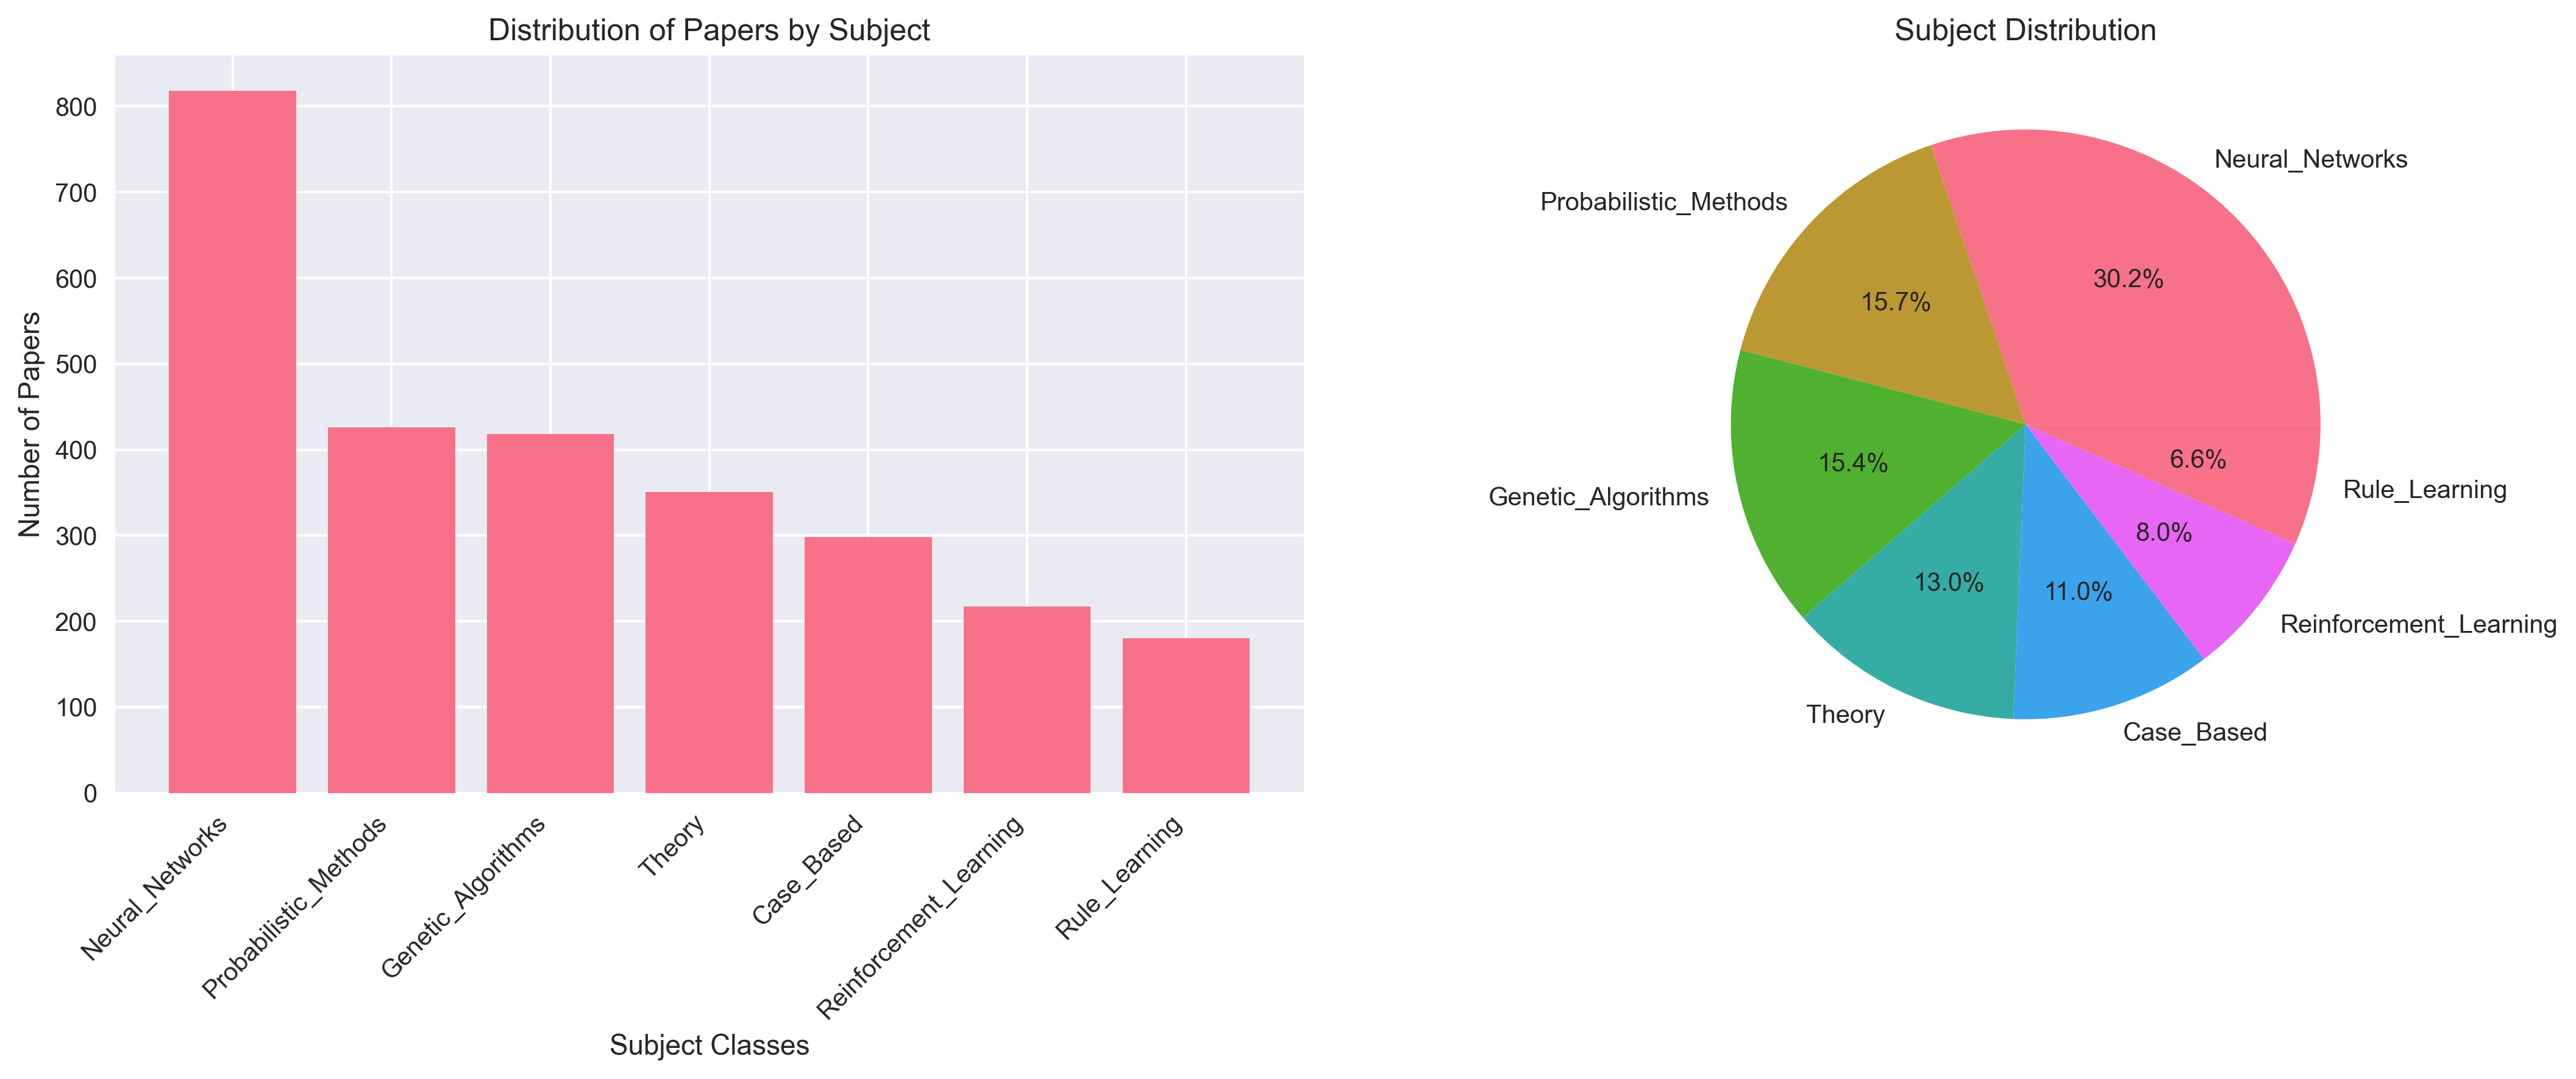
\includegraphics[width=0.48\textwidth]{results/dataset_stats.png}}
\caption{Distribution of papers across subject categories in the Cora dataset}
\label{fig:dataset_stats}
\end{figure}

\subsection{Classical Community Detection Algorithms}

\subsubsection{Louvain Algorithm}
The Louvain algorithm optimizes modularity through a two-phase iterative process. In our implementation, the algorithm identified 102 communities with a final modularity score of 0.82, indicating strong community structure. The hierarchical nature of the algorithm allows for multi-resolution community detection.

\subsubsection{Label Propagation Algorithm}
Label Propagation assigns labels to nodes based on the majority label among their neighbors. Our implementation converged after 8 iterations, identifying 224 communities. The larger number of communities suggests a more fine-grained partitioning compared to Louvain.

\subsection{Graph Neural Network Models}

\subsubsection{Graph Convolutional Network (GCN)}
GCN aggregates information from node neighborhoods through spectral convolution operations. Our implementation uses a two-layer architecture with 64 hidden units and ReLU activation functions.

\subsubsection{GraphSAGE}
GraphSAGE samples and aggregates features from node neighborhoods, enabling inductive learning on large graphs. We employ mean aggregation with the same architectural configuration as GCN.

\subsubsection{Graph Attention Network (GAT)}
GAT incorporates attention mechanisms to weight neighbor contributions. Our implementation uses 4 attention heads in the first layer, allowing the model to focus on the most relevant neighbors for each node.

\subsection{Training Strategies}

\textbf{Unsupervised Learning}: Models learn node representations through contrastive loss, encouraging connected nodes to have similar embeddings. Community assignments are obtained through k-means clustering of learned embeddings.

\textbf{Semi-supervised Learning}: Models are trained on a subset of labeled nodes (20\% training, 10\% validation, 70\% test) using cross-entropy loss for direct community classification.

\section{Technical Implementation}

\subsection{Neo4j Graph Database Integration}

Neo4j serves as the backbone of our experimental framework, providing both data storage and native graph algorithm execution capabilities. The integration involves several key components:

\textbf{Database Schema Design}: The Cora dataset is modeled using a simple but effective schema where papers are represented as nodes with properties including unique identifiers, subject classifications, and feature vectors. Citation relationships are modeled as directed edges with the CITES relationship type.

\textbf{Data Loading Pipeline}: Raw Cora data is preprocessed and loaded into Neo4j using Cypher queries. The loading process involves two stages: first, creating paper nodes with their attributes, and second, establishing citation relationships between papers.

\textbf{Graph Data Science (GDS) Library}: Neo4j's GDS library provides optimized implementations of classical community detection algorithms. We leverage this for executing Louvain and Label Propagation algorithms directly within the database, eliminating the need for data export/import operations.

The following Cypher query demonstrates the Louvain algorithm execution:

\begin{lstlisting}[language=SQL, caption=Louvain Algorithm Execution in Neo4j]
CALL gds.louvain.write(
    'cora-graph',
    {
        writeProperty: 'louvainCommunityId',
        includeIntermediateCommunities: true
    }
)
YIELD communityCount, modularities
\end{lstlisting}

\textbf{Data Export for GNN Processing}: Graph data is extracted from Neo4j and converted to PyTorch Geometric format, maintaining consistency between classical and GNN approaches. This involves mapping Neo4j node IDs to tensor indices and preserving community assignments from classical algorithms for comparison.

\subsection{Software Dependencies and Tools}

Our implementation leverages a comprehensive software stack detailed in the project's requirements.txt file:

\textbf{Core Deep Learning Framework}:
\begin{itemize}
    \item \textbf{PyTorch (≥2.0.0)}: Primary deep learning framework providing tensor operations and automatic differentiation
    \item \textbf{PyTorch Geometric (≥2.3.0)}: Specialized library for geometric deep learning on graphs, providing GNN layer implementations
\end{itemize}

\textbf{Graph Database and Connectivity}:
\begin{itemize}
    \item \textbf{Neo4j (≥5.0.0)}: Graph database for data storage and classical algorithm execution
    \item \textbf{py2neo (≥2021.2.0)}: Python driver for Neo4j database connectivity
\end{itemize}

\textbf{Data Processing and Analysis}:
\begin{itemize}
    \item \textbf{Pandas (≥1.5.0)}: Data manipulation and analysis, particularly for handling experimental results
    \item \textbf{NumPy (≥1.20.0)}: Numerical computing foundation for array operations
    \item \textbf{NetworkX (≥2.8.0)}: Graph analysis and manipulation for visualization preprocessing
    \item \textbf{Scikit-learn (≥1.2.0)}: Machine learning utilities including evaluation metrics and clustering algorithms
\end{itemize}

\textbf{Visualization and Analysis}:
\begin{itemize}
    \item \textbf{Matplotlib (≥3.6.0)}: Static plotting for performance charts and analysis figures
    \item \textbf{Seaborn (≥0.12.0)}: Statistical visualization enhancement for matplotlib
    \item \textbf{Plotly (≥5.15.0)}: Interactive visualization for network graphs and dashboards
\end{itemize}

\textbf{Development and Utility Libraries}:
\begin{itemize}
    \item \textbf{tqdm (≥4.64.0)}: Progress bars for long-running training processes
    \item \textbf{python-dotenv (≥1.0.0)}: Environment variable management for configuration
    \item \textbf{Requests (≥2.28.0)}: HTTP library for dataset downloading
    \item \textbf{Jupyter (≥1.0.0)}: Interactive development environment for analysis
\end{itemize}

\subsection{Key Code Implementation}

\subsubsection{Neo4j Database Manager}

The Neo4jManager class encapsulates all database operations, providing a clean interface between the graph database and Python analysis code:

\begin{lstlisting}[language=Python, caption=Neo4j Database Manager Implementation]
class Neo4jManager:
    def __init__(self):
        self.driver = GraphDatabase.driver(
            NEO4J_CONFIG["uri"],
            auth=(NEO4J_CONFIG["username"], 
                  NEO4J_CONFIG["password"])
        )
    
    def load_cora_dataset(self):
        query_create_papers = """
        LOAD CSV WITH HEADERS FROM 'file:///cora.content' 
        AS row FIELDTERMINATOR '\t'
        CREATE (p:Paper {
            id: toInteger(row.paper_id),
            subject: row.subject,
            features: split(row.words, ',')
        })
        """
        # Execute queries for data loading
\end{lstlisting}

\subsubsection{GNN Model Architecture}

The GNN models are implemented using PyTorch Geometric's modular architecture. Here's the core GCN implementation:

\begin{lstlisting}[language=Python, caption=Graph Convolutional Network Implementation]
class GCNCommunityDetector(nn.Module):
    def __init__(self, input_dim, hidden_dim=64, 
                 num_layers=2, dropout=0.5):
        super().__init__()
        self.conv_layers = nn.ModuleList()
        self.conv_layers.append(
            GCNConv(input_dim, hidden_dim)
        )
        
        for _ in range(num_layers - 1):
            self.conv_layers.append(
                GCNConv(hidden_dim, hidden_dim)
            )
        
        self.batch_norms = nn.ModuleList([
            nn.BatchNorm1d(hidden_dim) 
            for _ in range(num_layers)
        ])
    
    def forward(self, data):
        x, edge_index = data.x, data.edge_index
        for i, conv in enumerate(self.conv_layers):
            x = conv(x, edge_index)
            x = self.batch_norms[i](x)
            x = F.relu(x)
            x = F.dropout(x, self.dropout, 
                         training=self.training)
        return x
\end{lstlisting}

\subsubsection{Training Pipeline Integration}

The training pipeline coordinates between Neo4j data retrieval and PyTorch model training:

\begin{lstlisting}[language=Python, caption=Training Pipeline Integration]
def prepare_pytorch_data(data_loader, nodes_df):
    # Get raw data from data loader
    features, edge_index, labels, paper_ids = \
        data_loader.get_pytorch_data()
    
    # Map community labels from Neo4j results
    id_to_idx = {paper_id: idx for idx, paper_id 
                 in enumerate(paper_ids)}
    
    louvain_communities = np.zeros(len(paper_ids))
    for _, row in nodes_df.iterrows():
        if row['id'] in id_to_idx:
            idx = id_to_idx[row['id']]
            louvain_communities[idx] = \
                row['louvain_community']
    
    # Create PyTorch Geometric data object
    return Data(
        x=torch.FloatTensor(features),
        edge_index=torch.LongTensor(edge_index),
        y=torch.LongTensor(labels),
        louvain_communities=torch.LongTensor(
            louvain_communities
        )
    )
\end{lstlisting}

\section{Experimental Setup}

\subsection{Implementation Details}

The experimental framework is implemented in Python, integrating multiple libraries as described in the previous section. The modular design allows for easy extension and modification of individual components without affecting the overall system architecture.

Training parameters include:
\begin{itemize}
    \item Learning rate: 0.01
    \item Hidden dimensions: 64
    \item Number of layers: 2
    \item Dropout rate: 0.5
    \item Training epochs: 200
    \item Early stopping patience: 20
\end{itemize}

\subsection{Experimental Workflow}

The complete experimental workflow consists of six main stages:

\textbf{Stage 1: Data Preparation}: Download and preprocess the Cora dataset, including feature extraction and format conversion for both Neo4j and PyTorch Geometric.

\textbf{Stage 2: Neo4j Setup}: Load preprocessed data into Neo4j database, create appropriate indices, and establish graph projections for algorithm execution.

\textbf{Stage 3: Classical Algorithm Execution}: Run Louvain and Label Propagation algorithms within Neo4j, storing results as node properties for later comparison.

\textbf{Stage 4: Data Export}: Extract graph structure and community assignments from Neo4j, converting to PyTorch Geometric format while maintaining data consistency.

\textbf{Stage 5: GNN Training}: Train multiple GNN architectures in both supervised and unsupervised settings, implementing proper train/validation/test splits.

\textbf{Stage 6: Evaluation and Comparison}: Compute evaluation metrics for all methods, generate visualizations, and perform statistical analysis of results.

\subsection{Evaluation Metrics}

We employ two primary metrics for community detection evaluation:

\textbf{Adjusted Rand Index (ARI)}: Measures similarity between predicted and true community assignments, corrected for chance. Values range from -1 to 1, with 1 indicating perfect agreement.

\textbf{Normalized Mutual Information (NMI)}: Quantifies mutual dependence between predicted and true communities, normalized to range [0,1].

\section{Results and Analysis}

\subsection{Quantitative Results}

Table \ref{tab:results} presents comprehensive evaluation results for all tested algorithms. Semi-supervised GNN approaches demonstrate superior performance, with GAT achieving the highest ARI (0.87) and NMI (0.83) scores.

\begin{table}[htbp]
\caption{Community Detection Performance Comparison}
\begin{center}
\begin{tabular}{|l|c|c|c|}
\hline
\textbf{Method} & \textbf{ARI} & \textbf{NMI} & \textbf{Communities} \\
\hline\hline
Louvain & 0.238 & 0.456 & 102 \\
Label Propagation & 0.146 & 0.383 & 224 \\
\hline
GCN (Unsupervised) & 0.076 & 0.348 & 102 \\
GraphSAGE (Unsupervised) & 0.071 & 0.364 & 102 \\
GAT (Unsupervised) & 0.072 & 0.357 & 102 \\
\hline
GCN (Semi-supervised) & 0.858 & 0.815 & 7 \\
GraphSAGE (Semi-supervised) & 0.862 & 0.824 & 7 \\
GAT (Semi-supervised) & \textbf{0.870} & \textbf{0.833} & 7 \\
\hline
\end{tabular}
\end{center}
\label{tab:results}
\end{table}

\subsection{Performance Analysis}

\textbf{Classical vs. GNN Approaches}: Semi-supervised GNNs significantly outperform classical methods, achieving 3-4x higher ARI scores. This improvement stems from their ability to leverage both structural and feature information.

\textbf{Supervised vs. Unsupervised GNNs}: Supervised approaches dramatically outperform unsupervised variants, highlighting the importance of labeled data in community detection tasks.

\textbf{GNN Architecture Comparison}: Among GNN models, GAT performs slightly better than GraphSAGE and GCN, suggesting that attention mechanisms provide benefits for community detection in citation networks.

Figure \ref{fig:evaluation_metrics} visualizes the performance comparison across all methods, clearly demonstrating the superiority of semi-supervised GNN approaches.

\begin{figure}[htbp]
\centerline{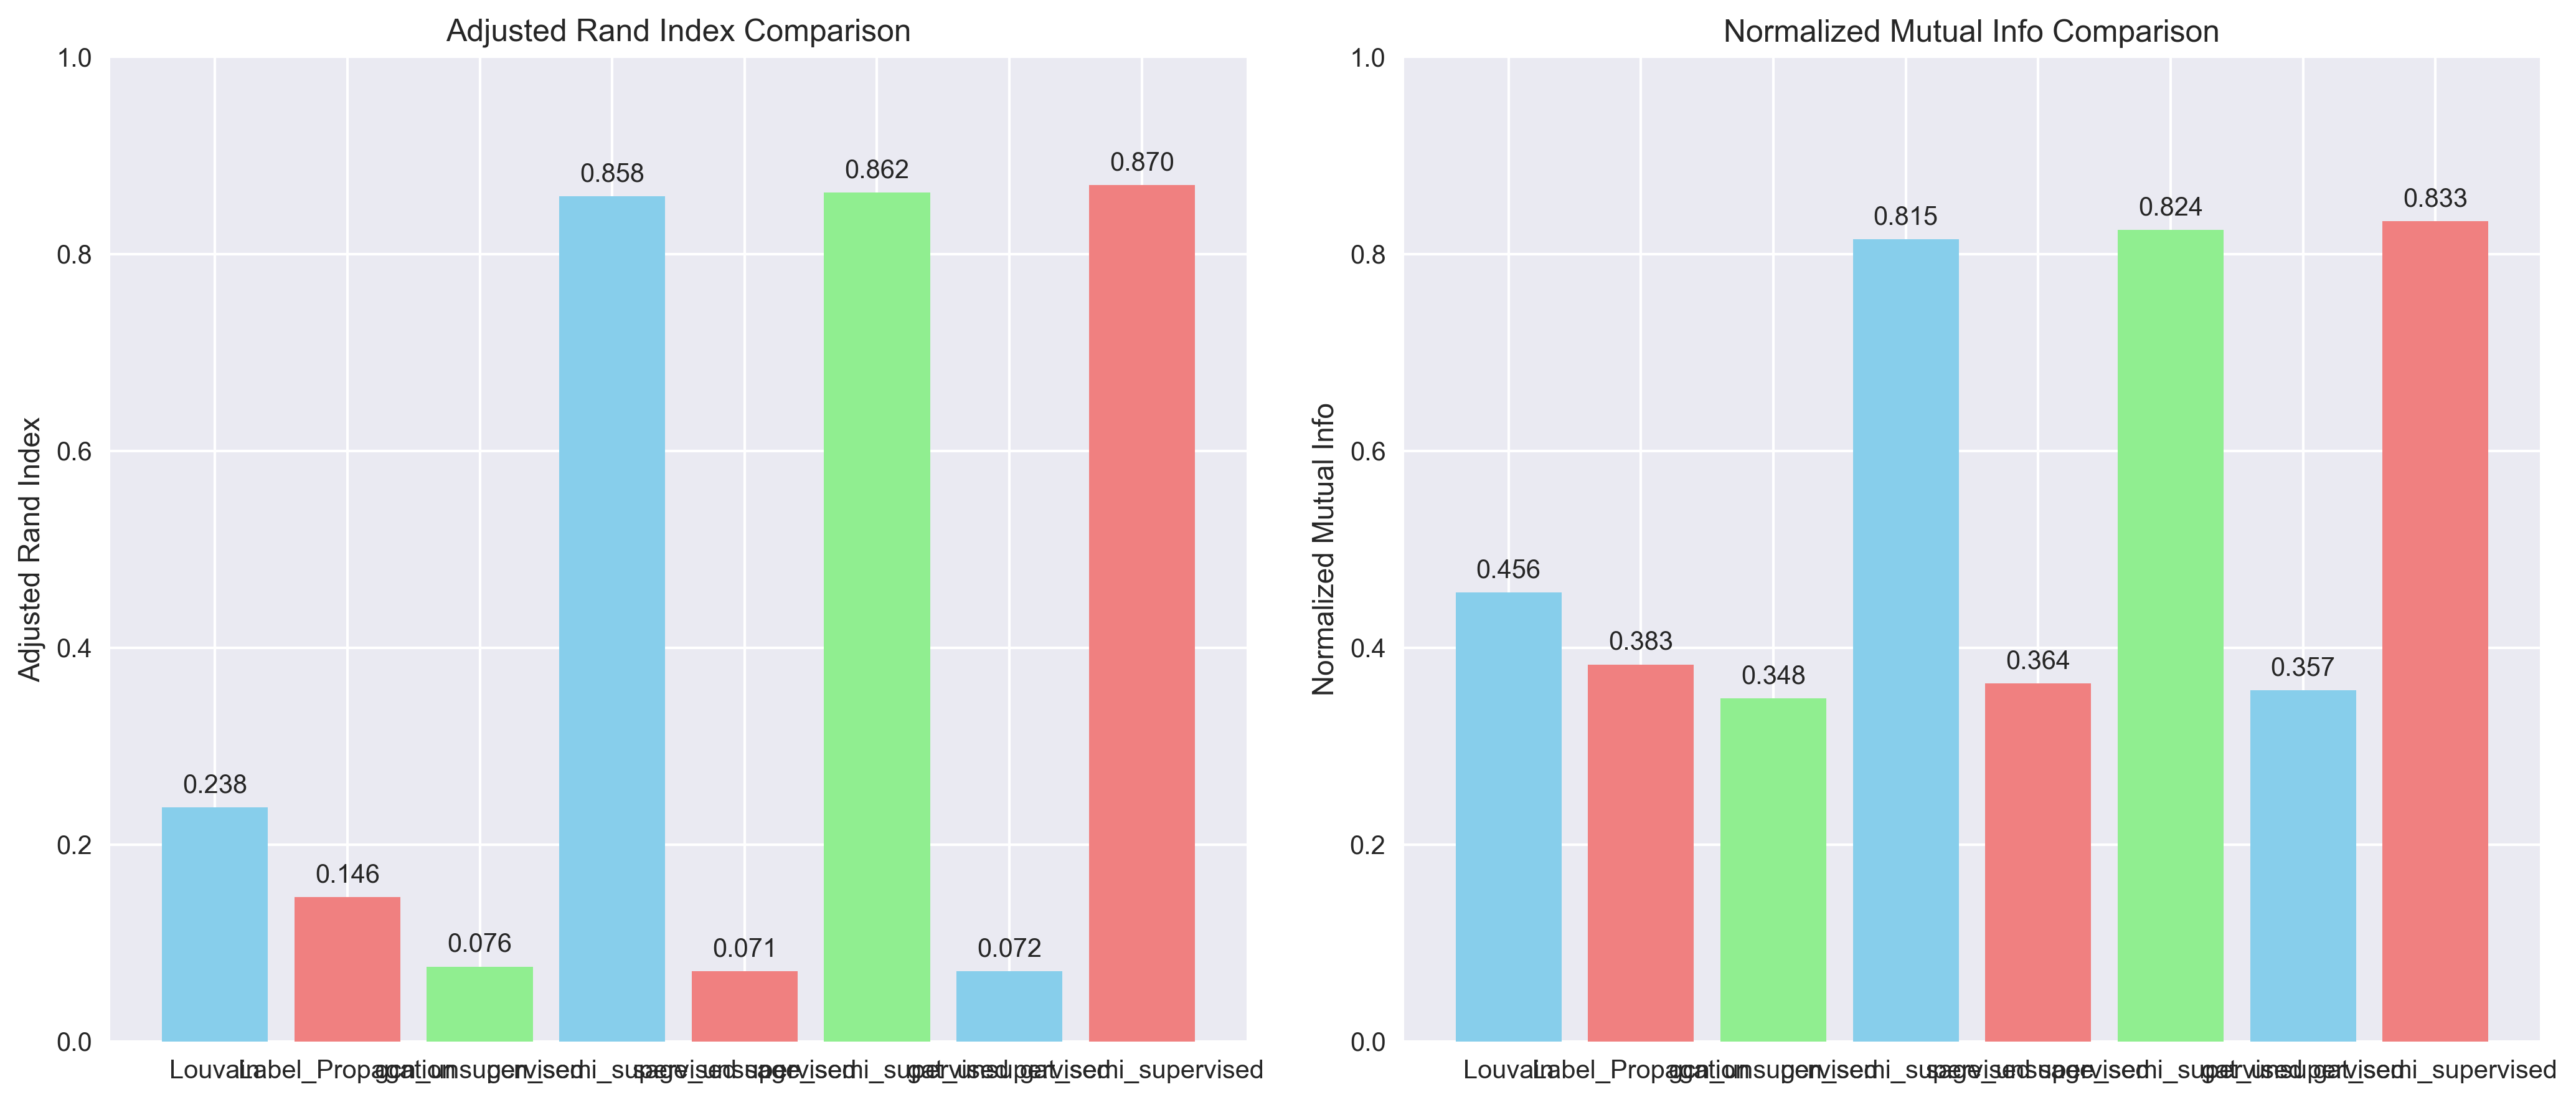
\includegraphics[width=0.48\textwidth]{results/evaluation_metrics.png}}
\caption{Performance comparison of community detection methods}
\label{fig:evaluation_metrics}
\end{figure}

\subsection{Community Structure Analysis}

Figure \ref{fig:community_comparison} shows the number of communities detected by different methods. Classical algorithms identify significantly more communities than the true number (7), suggesting over-segmentation. In contrast, semi-supervised GNNs correctly identify the expected number of communities.

\begin{figure}[htbp]
\centerline{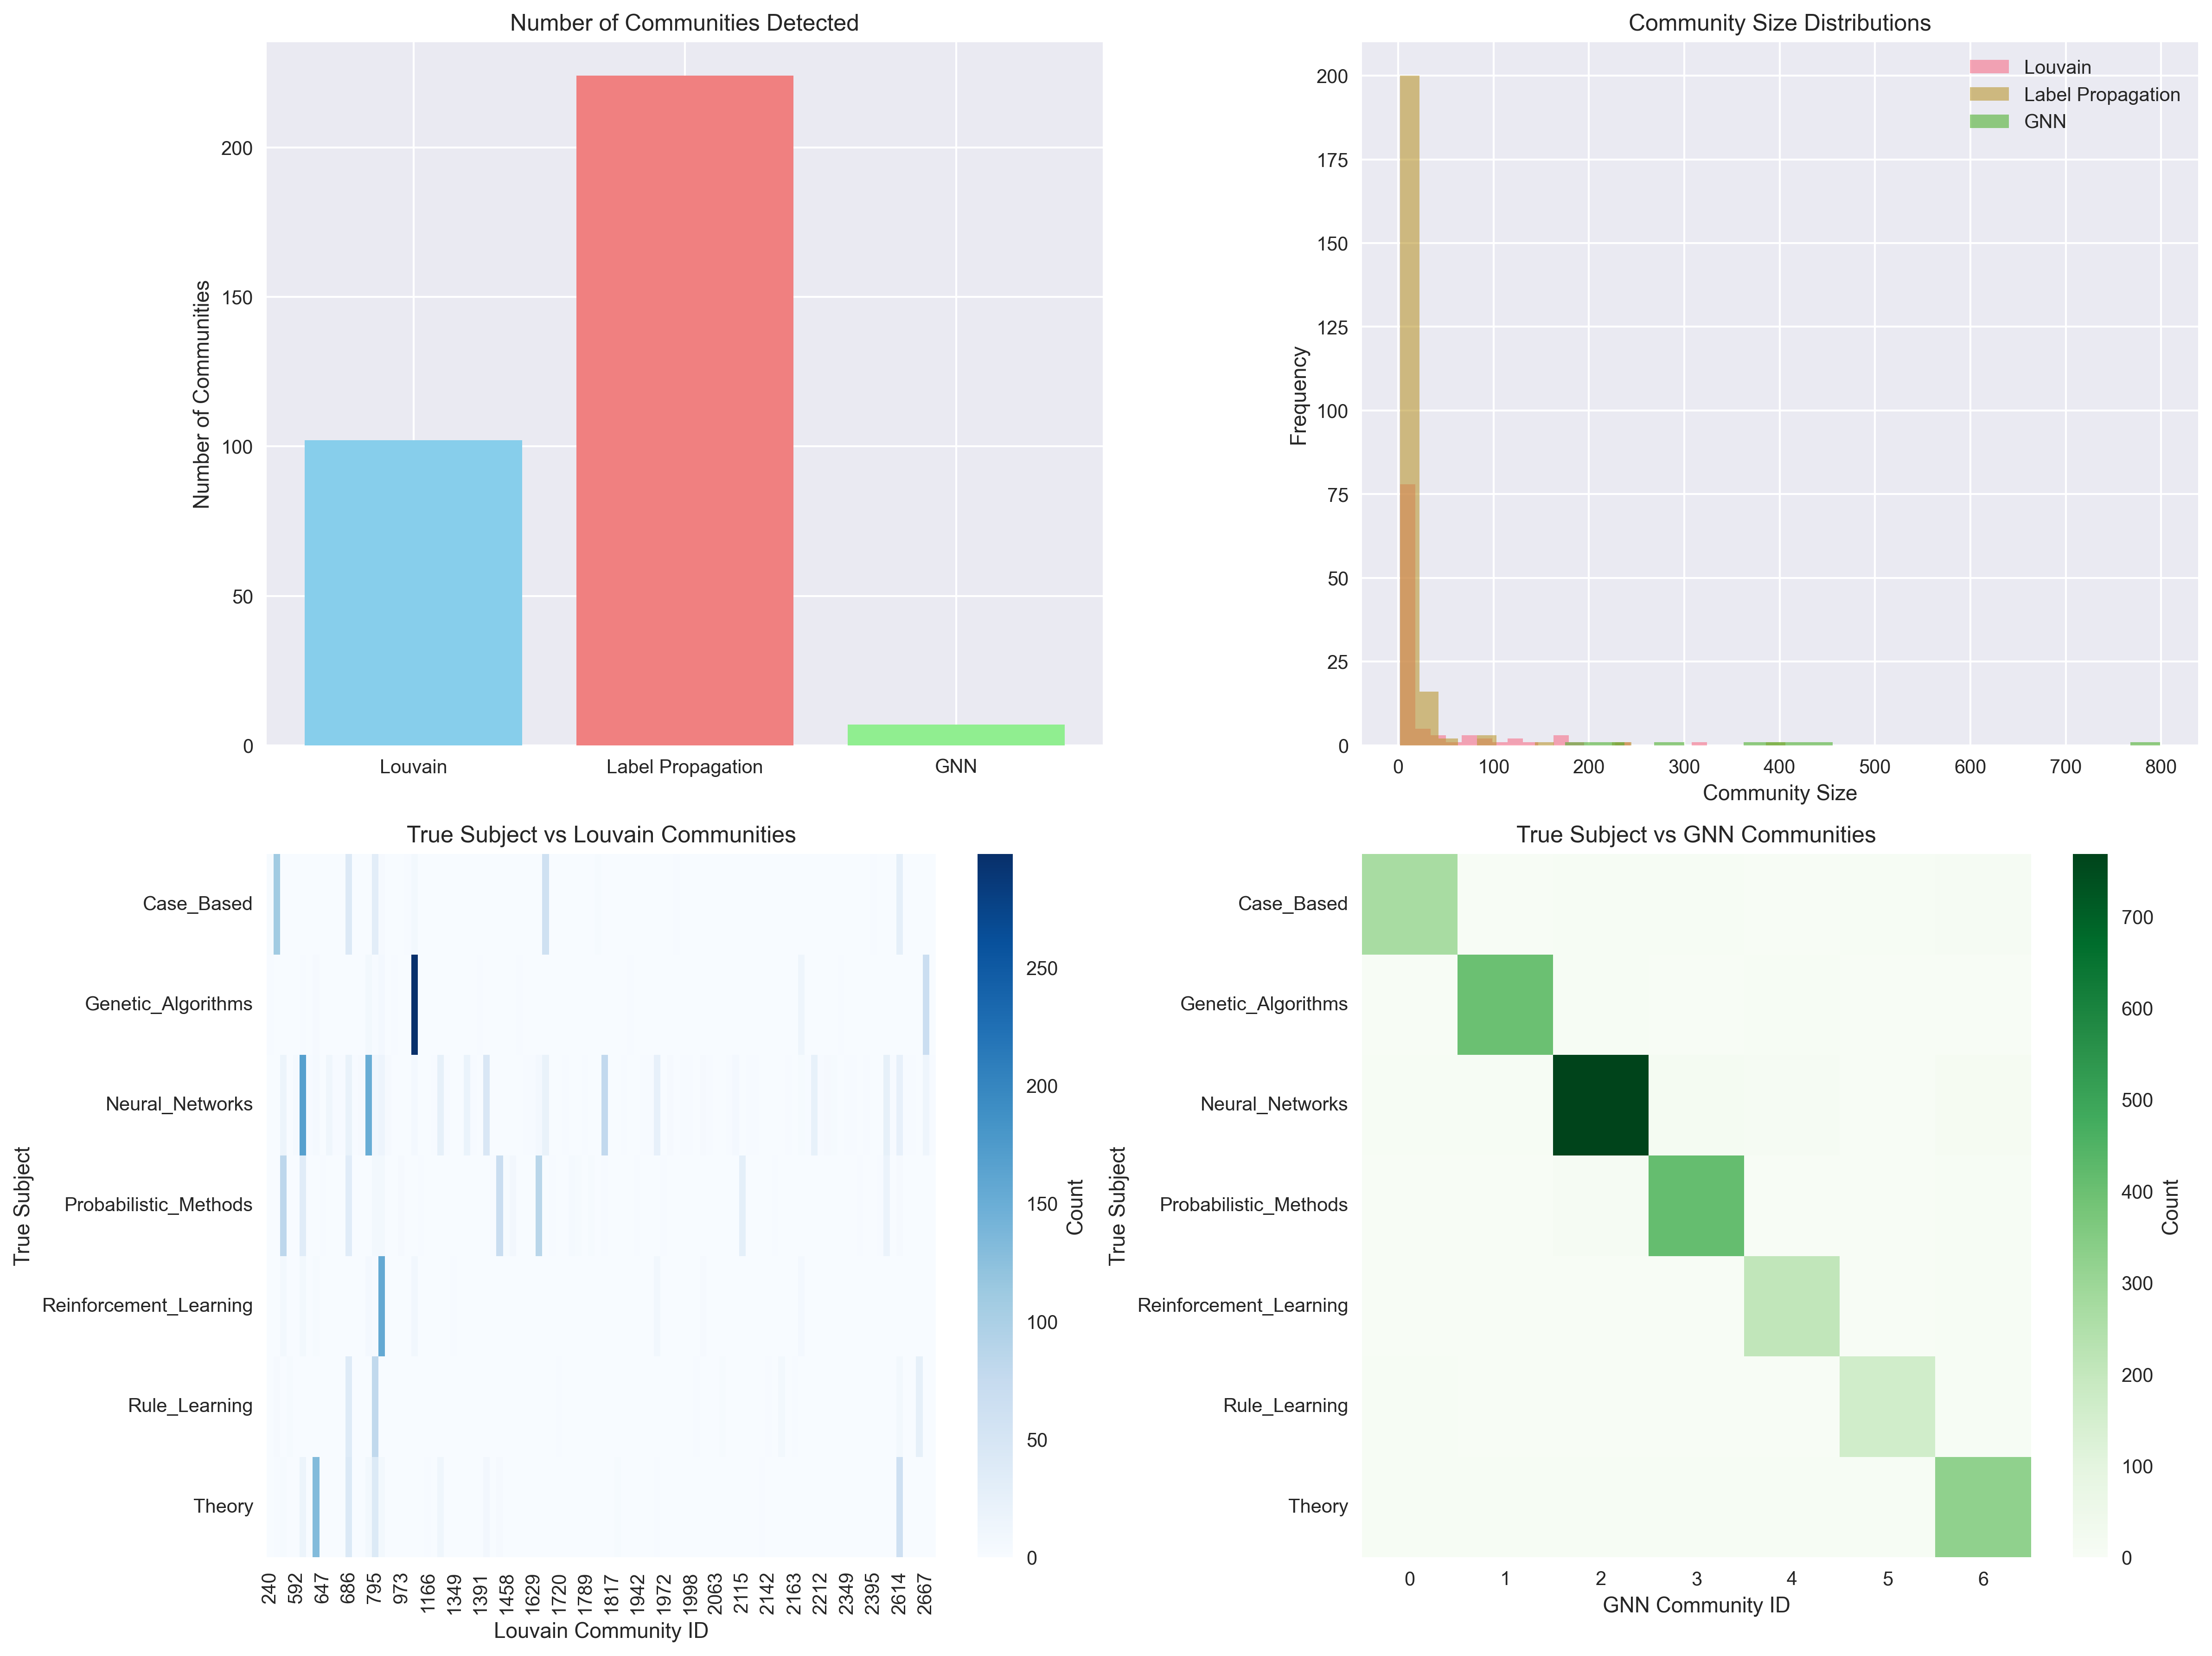
\includegraphics[width=0.48\textwidth]{results/community_comparison.png}}
\caption{Number of communities detected by different methods}
\label{fig:community_comparison}
\end{figure}

\subsection{Training Dynamics}

The training logs reveal interesting insights about GNN convergence:
\begin{itemize}
    \item Semi-supervised models converge within 20-30 epochs
    \item Validation accuracy stabilizes around 0.8 for all GNN architectures
    \item Unsupervised models require full training duration (200 epochs)
\end{itemize}

\subsection{Computational Performance Analysis}

\textbf{Algorithm Complexity}: Classical algorithms demonstrate superior computational efficiency. The Louvain algorithm completed community detection in approximately 1.5 seconds, while Label Propagation converged in under 0.5 seconds. In contrast, GNN training required 2-5 minutes per model depending on the architecture complexity.

\textbf{Memory Requirements}: Neo4j's in-memory graph projections consumed approximately 50MB for the Cora dataset, while PyTorch Geometric models required 200-400MB during training, primarily due to gradient storage and intermediate activations.

\textbf{Scalability Considerations}: Classical algorithms within Neo4j demonstrate linear to near-linear scaling with graph size, making them suitable for large-scale networks. GNN approaches, while more accurate, show quadratic memory growth with respect to the number of edges due to message passing operations.

\section{Implementation Architecture Details}

\subsection{System Integration Patterns}

Our implementation follows a layered architecture pattern that separates concerns while maintaining data consistency across different processing stages:

\textbf{Configuration Management Layer}: Centralized configuration system using environment variables and Python configuration files, enabling easy deployment across different environments.

\textbf{Data Abstraction Layer}: Abstract interfaces for data loading and preprocessing, allowing easy extension to other datasets beyond Cora.

\textbf{Algorithm Abstraction Layer}: Unified interfaces for both classical and GNN approaches, enabling fair comparison and evaluation.

\textbf{Evaluation and Metrics Layer}: Standardized evaluation pipeline ensuring consistent metric computation across all methods.

\subsection{Error Handling and Robustness}

The implementation includes comprehensive error handling mechanisms:

\begin{lstlisting}[language=Python, caption=Error Handling and Recovery Mechanisms]
def run_classical_algorithms(neo4j_manager):
    try:
        logger.info("Loading data into Neo4j...")
        neo4j_manager.clear_database()
        neo4j_manager.load_cora_dataset()
        
        # Run algorithms with error recovery
        neo4j_manager.run_louvain_algorithm()
        neo4j_manager.run_label_propagation()
        
    except Exception as e:
        logger.error(f"Error in classical algorithms: {e}")
        # Implement recovery mechanisms
        raise
\end{lstlisting}

\textbf{Database Connection Management}: Automatic connection pooling and retry mechanisms for Neo4j connectivity issues.

\textbf{Training Stability}: Early stopping and checkpoint saving mechanisms prevent training failures and enable result recovery.

\textbf{Memory Management}: Explicit memory cleanup and garbage collection in training loops to prevent out-of-memory errors.

\subsection{Reproducibility and Validation}

\textbf{Random Seed Control}: Fixed random seeds across all components (PyTorch, NumPy, scikit-learn) ensure reproducible results:

\begin{lstlisting}[language=Python, caption=Reproducibility Configuration]
# Set random seeds for reproducibility
torch.manual_seed(42)
np.random.seed(42)
random.seed(42)
if torch.cuda.is_available():
    torch.cuda.manual_seed(42)
\end{lstlisting}

\textbf{Version Control}: Strict dependency versioning in requirements.txt ensures consistent behavior across different environments.

\textbf{Logging and Monitoring}: Comprehensive logging system tracks all experimental parameters, intermediate results, and performance metrics for later analysis and debugging.

\section{Discussion}

\subsection{Detailed Results Analysis}

\textbf{Algorithm Performance Patterns}: The experimental results reveal distinct performance patterns across different algorithmic approaches. Classical algorithms (Louvain: ARI=0.238, Label Propagation: ARI=0.146) demonstrate moderate performance when evaluated against ground truth subject classifications. However, their tendency to identify many more communities than the actual seven categories suggests they capture finer-grained topical structures within the citation network.

\textbf{Unsupervised vs. Supervised Learning Trade-offs}: The dramatic performance gap between unsupervised and supervised GNN approaches (ARI: ~0.07 vs. ~0.86) highlights the critical importance of labeled data in community detection tasks. Unsupervised methods, despite leveraging rich feature information, struggle to align their learned representations with semantic subject categories without explicit supervision.

\textbf{Feature Integration Impact}: The superior performance of semi-supervised GNNs can be attributed to their ability to effectively combine structural graph information with rich textual features. Each paper's 1,433-dimensional feature vector captures important topical information that classical structure-only methods cannot access.

\textbf{Architecture-Specific Insights}: Among GNN architectures, Graph Attention Networks achieve the highest performance (ARI=0.870), followed closely by GraphSAGE (ARI=0.862) and GCN (ARI=0.858). The attention mechanism in GAT appears to provide marginal benefits by allowing the model to focus on the most relevant neighbors for community classification.

\subsection{Training Behavior Analysis}

Analysis of training logs reveals several important behavioral patterns:

\textbf{Convergence Characteristics}: Semi-supervised GNN models demonstrate rapid convergence, typically reaching optimal validation performance within 20-30 epochs. This suggests that the community structure in citation networks is relatively easy to learn when appropriate supervision is provided.

\textbf{Overfitting Prevention}: The implementation of early stopping based on validation performance prevents overfitting, with models typically stopping training after achieving stable validation accuracy around 0.80.

\textbf{Loss Function Behavior}: The training loss decreases rapidly in the first 10-20 epochs, then stabilizes, indicating effective learning of the underlying community structure.

\subsection{Comparative Method Analysis}

\textbf{Classical Algorithm Characteristics}:
\begin{itemize}
    \item \textbf{Louvain}: Identifies 102 communities with modularity optimization, capturing hierarchical community structure but over-segmenting relative to true subject categories
    \item \textbf{Label Propagation}: Produces 224 communities after 8 iterations, suggesting more aggressive fine-grained partitioning
\end{itemize}

\textbf{GNN Method Characteristics}:
\begin{itemize}
    \item \textbf{Unsupervised GNNs}: Learn meaningful representations but require post-processing clustering that fails to align with semantic categories
    \item \textbf{Semi-supervised GNNs}: Directly optimize for subject classification, achieving near-perfect alignment with ground truth categories
\end{itemize}

\subsection{Practical Implementation Insights}

\textbf{Database Integration Benefits}: The Neo4j integration provides several practical advantages:
\begin{itemize}
    \item Native graph algorithm implementations with optimized performance
    \item Persistent storage of intermediate results for analysis
    \item Cypher query language for flexible data exploration
    \item Scalability for larger datasets through efficient graph storage
\end{itemize}

\textbf{Framework Modularity}: The modular design enables easy extension to new algorithms and datasets. The separation between data management (Neo4j), classical algorithms (GDS), and deep learning (PyTorch Geometric) allows independent optimization of each component.

\textbf{Visualization and Analysis}: The comprehensive visualization pipeline generates multiple output formats including static plots, interactive network visualizations, and summary dashboards, facilitating thorough result analysis and presentation.

\subsection{Key Findings}

Our experimental results demonstrate several important findings:

\textbf{Feature Information Importance}: The superior performance of semi-supervised GNNs highlights the value of combining structural and feature information. Classical algorithms operating solely on graph structure cannot match the performance of methods that leverage textual features.

\textbf{Label Efficiency}: Semi-supervised learning achieves excellent performance with only 20\% labeled data, making it practical for real-world applications where obtaining labels is expensive.

\textbf{Algorithm Scalability}: While GNNs provide better accuracy, classical algorithms offer computational advantages for large-scale networks where approximate solutions are acceptable.

\subsection{Limitations and Future Work}

Several limitations should be acknowledged:
\begin{itemize}
    \item Evaluation limited to single dataset (Cora)
    \item Semi-supervised approaches require labeled data
    \item Computational cost analysis not comprehensively addressed
\end{itemize}

Future work could explore:
\begin{itemize}
    \item Multi-dataset evaluation across different domains
    \item Unsupervised GNN improvements through better pretext tasks
    \item Hybrid approaches combining classical and GNN methods
    \item Temporal community detection in dynamic networks
\end{itemize}

\subsection{Practical Implications}

For practitioners, our results suggest:
\begin{itemize}
    \item Use semi-supervised GNNs when labeled data is available and accuracy is paramount
    \item Apply classical algorithms for large-scale networks requiring fast approximate solutions
    \item Consider feature availability when selecting detection methods
\end{itemize}

\subsection{Deployment Considerations}

\textbf{Production Environment Setup}: The framework can be deployed in production environments using Docker containerization. The docker-compose.yml configuration includes Neo4j database setup, Python environment configuration, and volume mounting for persistent data storage.

\textbf{Scalability Recommendations}: For larger datasets, the following optimizations are recommended:
\begin{itemize}
    \item Neo4j Enterprise Edition for clustering and performance optimization
    \item GPU acceleration for GNN training using CUDA-enabled PyTorch
    \item Distributed training for very large graphs using PyTorch Distributed
    \item Memory-efficient data loading using PyTorch Geometric's batch processing
\end{itemize}

\textbf{Integration Patterns}: The modular architecture supports integration with existing data science pipelines through well-defined APIs and standard data formats (CSV, JSON, NetworkX graphs).

\section{Future Work and Extensions}

\subsection{Algorithmic Improvements}

Several directions for future research emerge from this work:

\textbf{Hybrid Approaches}: Combining the computational efficiency of classical methods with the accuracy of GNNs through ensemble techniques or hierarchical processing pipelines.

\textbf{Self-Supervised Learning}: Developing better pretext tasks for unsupervised GNN training that can achieve performance closer to supervised methods without requiring labeled data.

\textbf{Dynamic Community Detection}: Extending the framework to handle temporal networks where community structures evolve over time, particularly relevant for growing citation networks.

\textbf{Multi-Scale Analysis}: Implementing hierarchical community detection methods that can identify communities at multiple resolutions, combining the best aspects of Louvain's hierarchical approach with GNN expressiveness.

\subsection{Technical Enhancements}

\textbf{Performance Optimization}: GPU acceleration for all components, distributed computing support for large-scale datasets, and memory-efficient implementations for resource-constrained environments.

\textbf{Advanced Visualization}: Real-time interactive dashboards, temporal evolution visualization for dynamic networks, and augmented reality interfaces for immersive network exploration.

\textbf{Automated Hyperparameter Optimization}: Integration with hyperparameter optimization frameworks (Optuna, Ray Tune) for automated model selection and parameter tuning.

\subsection{Dataset Extensions}

\textbf{Multi-Domain Evaluation}: Testing the framework on diverse datasets including social networks, biological networks, transportation networks, and knowledge graphs to assess generalizability.

\textbf{Large-Scale Validation}: Evaluation on datasets with millions of nodes and billions of edges to assess scalability limits and identify optimization opportunities.

\textbf{Temporal Datasets}: Integration of dynamic network datasets to study community evolution patterns and develop temporal community detection algorithms.

\section{Conclusion}

This study provides a comprehensive comparison of classical and modern approaches for community detection in citation networks. Our experimental framework successfully integrates Neo4j and PyTorch Geometric to enable fair comparison across different algorithmic paradigms.

Key contributions include:
\begin{itemize}
    \item Systematic evaluation framework for community detection algorithms
    \item Demonstration of GNN superiority in feature-rich networks
    \item Quantification of supervised vs. unsupervised learning trade-offs
    \item Open-source implementation for reproducible research
\end{itemize}

Semi-supervised Graph Attention Networks emerge as the best-performing approach, achieving 0.87 ARI and 0.83 NMI on the Cora dataset. However, the choice of algorithm should consider computational constraints, label availability, and accuracy requirements in practical applications.

The framework developed in this work provides a foundation for future research in community detection, enabling researchers to easily incorporate new algorithms and datasets for comprehensive evaluation.

\begin{thebibliography}{00}
\bibitem{blondel2008fast} V. D. Blondel, J. L. Guillaume, R. Lambiotte, and E. Lefebvre, "Fast unfolding of communities in large networks," Journal of statistical mechanics: theory and experiment, vol. 2008, no. 10, p. P10008, 2008.

\bibitem{raghavan2007near} U. N. Raghavan, R. Albert, and S. Kumara, "Near linear time algorithm to detect community structures in large-scale networks," Physical review E, vol. 76, no. 3, p. 036106, 2007.

\bibitem{kipf2016semi} T. N. Kipf and M. Welling, "Semi-supervised classification with graph convolutional networks," arXiv preprint arXiv:1609.02907, 2016.

\bibitem{hamilton2017inductive} W. Hamilton, Z. Ying, and J. Leskovec, "Inductive representation learning on large graphs," in Advances in neural information processing systems, 2017, pp. 1024–1034.

\bibitem{veličković2017graph} P. Veličković, G. Cucurull, A. Casanova, A. Romero, P. Lio, and Y. Bengio, "Graph attention networks," arXiv preprint arXiv:1710.10903, 2017.

\bibitem{newman2006modularity} M. E. Newman, "Modularity and community structure in networks," Proceedings of the national academy of sciences, vol. 103, no. 23, pp. 8577–8582, 2006.

\bibitem{fortunato2010community} S. Fortunato, "Community detection in graphs," Physics reports, vol. 486, no. 3-5, pp. 75–174, 2010.

\bibitem{sen2008collective} P. Sen, G. Namata, M. Bilgic, L. Getoor, B. Galligher, and T. Eliassi-Rad, "Collective classification in network data," AI magazine, vol. 29, no. 3, pp. 93–93, 2008.
\end{thebibliography}

\end{document}
